\documentclass[xetex,mathsans,sans,aspectratio=169]{beamer}
\usepackage{listings}
\usetheme{Boadilla}
\usecolortheme{orchid}
\usepackage{fontspec}
\setsansfont{Basis Grotesque}
\setbeamertemplate{navigation symbols}{}
\usepackage{amsmath}
\usepackage{multicol}


\title[NuCypher]{
\includegraphics[width=5.5cm]{pdf/nucypher_logo.pdf}}
\author[Michael]{Michael Egorov}
\date[Sep 6]{ETH Security UnConference, 6 Sep 2018}

\begin{document}
    \begin{frame}
        \titlepage
    \end{frame}

    \begin{frame}
        \frametitle{Why}
        \framesubtitle{Sharing data while encrypted}
        \begin{figure}
            \centering
            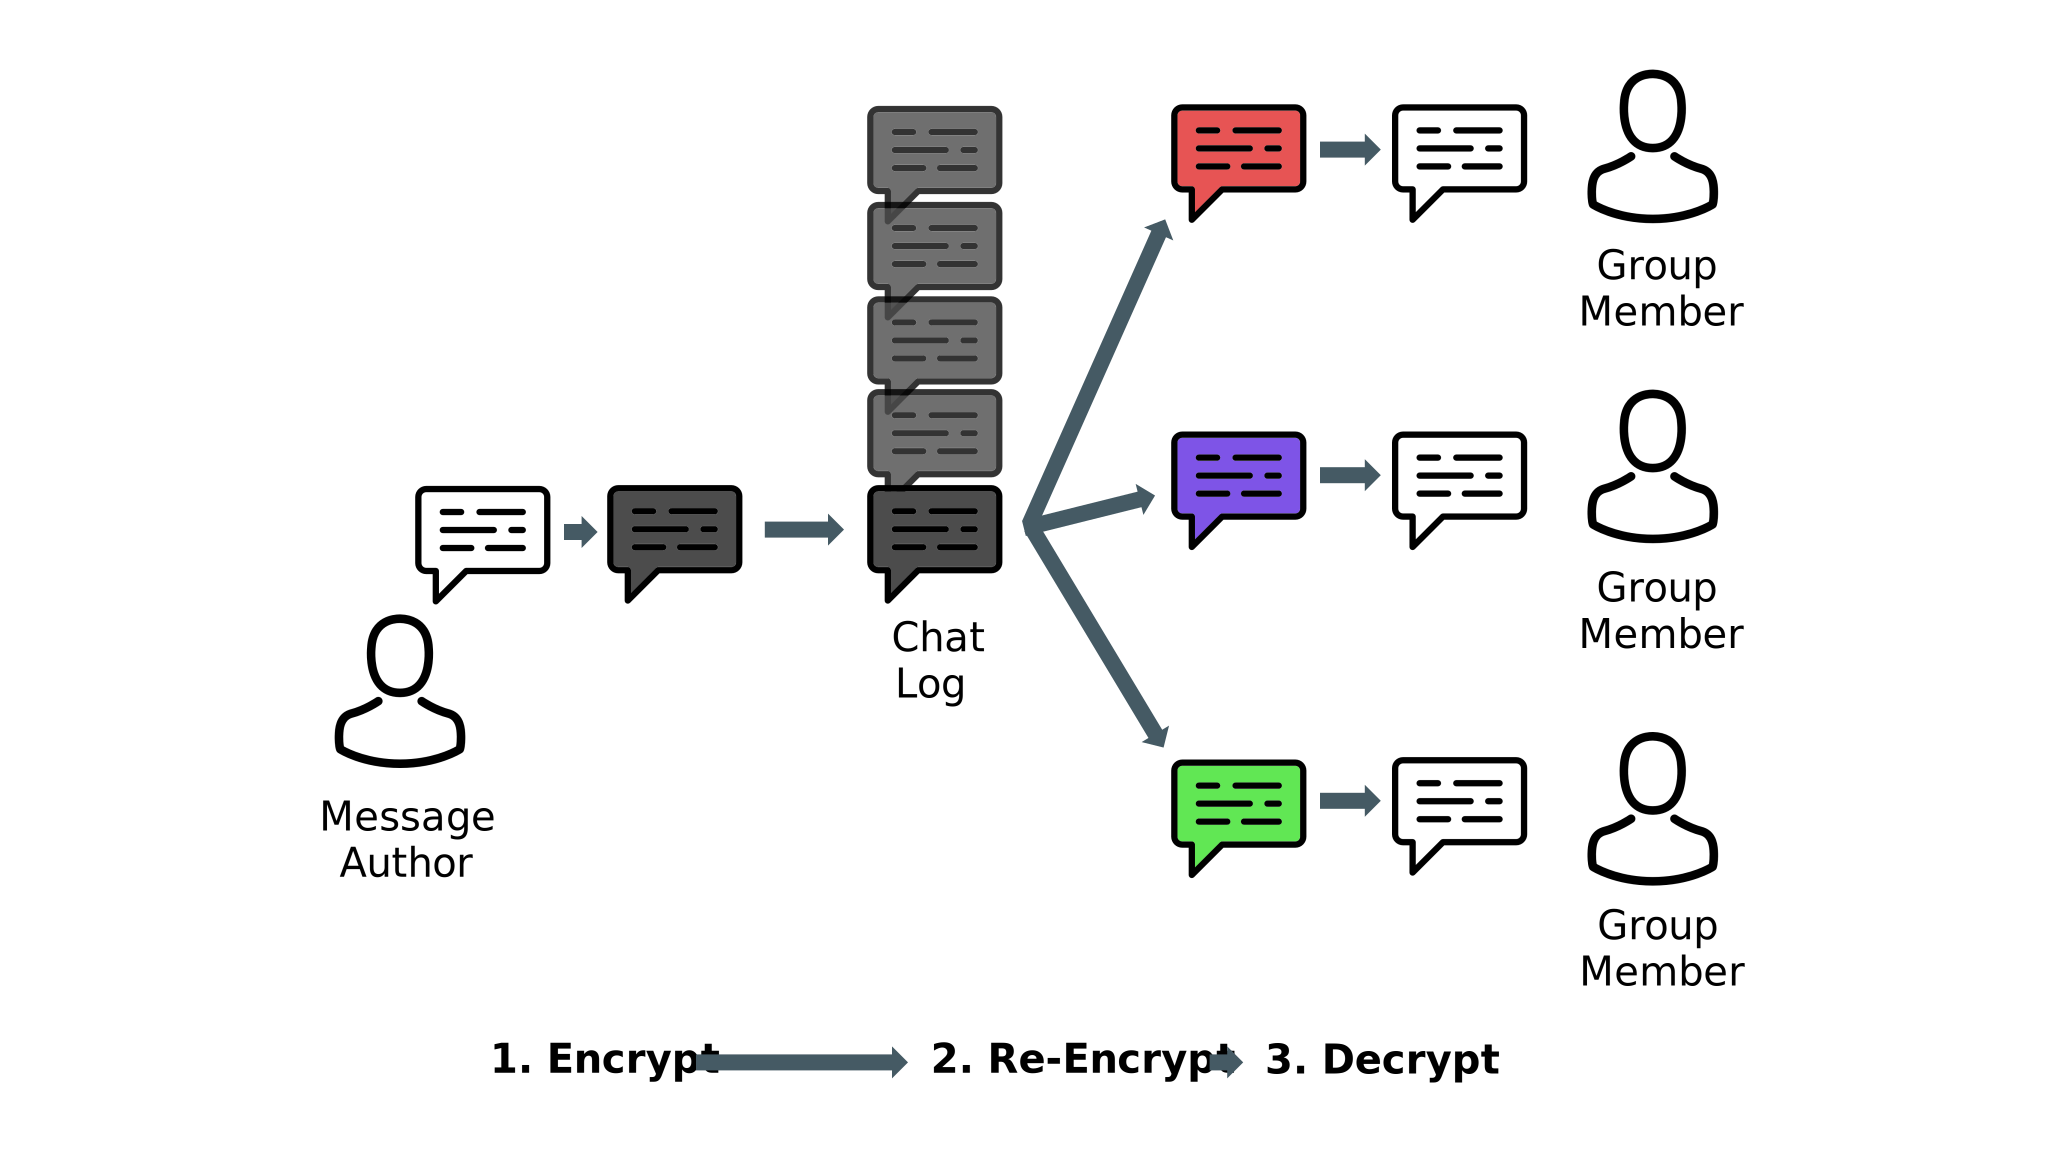
\includegraphics[height=5.5cm]{pdf/chats-alternative.pdf}
        \end{figure}
    \end{frame}

    \begin{frame}
        \frametitle{What is proxy re-encryption (PRE)}
        \begin{figure}
            \centering
            \includegraphics[width=11cm]{pdf/pre.pdf}
        \end{figure}
    \end{frame}

    \begin{frame}
        \frametitle{PRE and multiple receivers}
        \begin{figure}
            \centering
            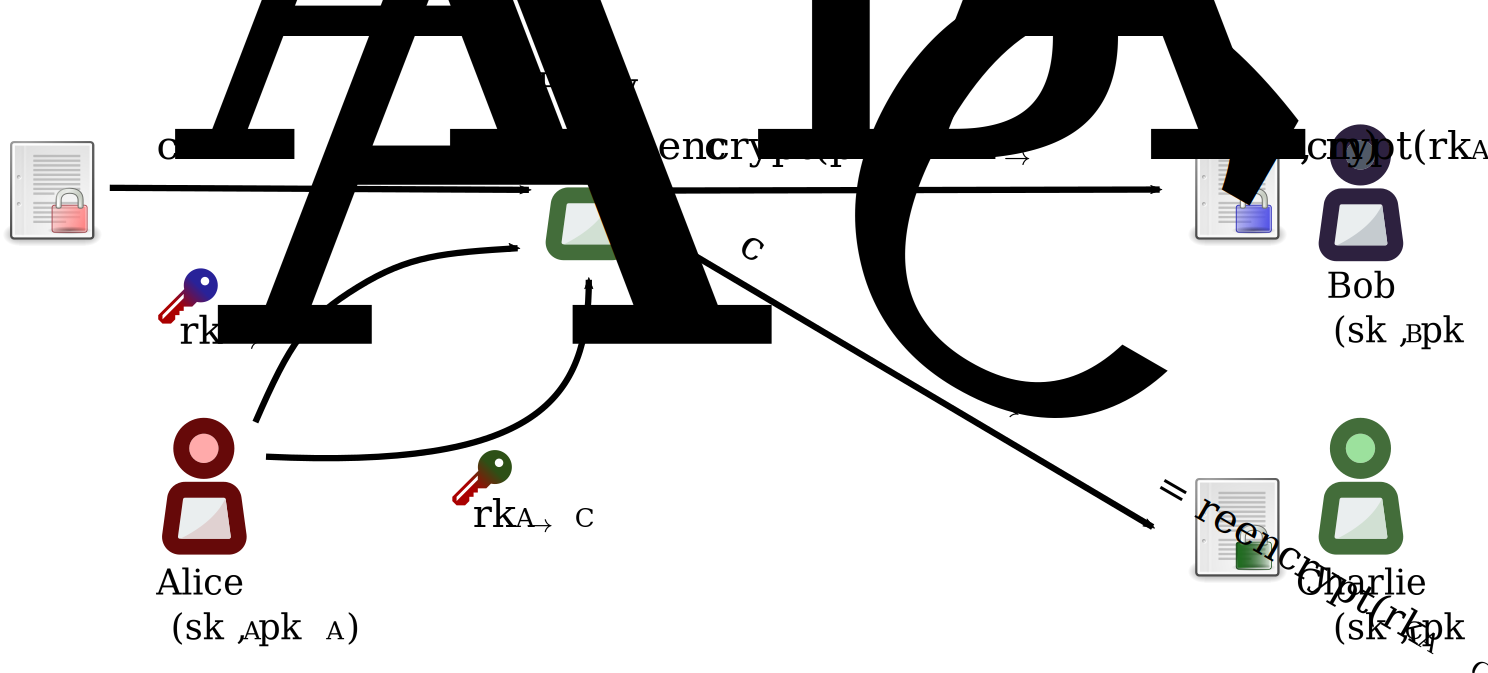
\includegraphics[width=11cm]{pdf/pre-multi.pdf}
        \end{figure}
    \end{frame}

    \begin{frame}
        \frametitle{Key management using PRE}
        \framesubtitle{Encryption}
        \begin{figure}
            \centering
            \includegraphics[height=5.5cm]{pdf/encrypt.pdf}
        \end{figure}
    \end{frame}

    \begin{frame}
        \frametitle{Key management using PRE}
        \framesubtitle{Access delegation}
        \begin{figure}
            \centering
            \includegraphics[height=5.5cm]{pdf/delegate.pdf}
        \end{figure}
    \end{frame}

    \begin{frame}
        \frametitle{Key management using PRE}
        \framesubtitle{Decryption}
        \begin{figure}
            \centering
            \includegraphics[height=5.5cm]{pdf/decrypt.pdf}
        \end{figure}
    \end{frame}

    \begin{frame}
        \frametitle{Decentralized key management}
        \framesubtitle{Using threshold split-key re-encryption (Umbral)}
        \begin{figure}
            \centering
            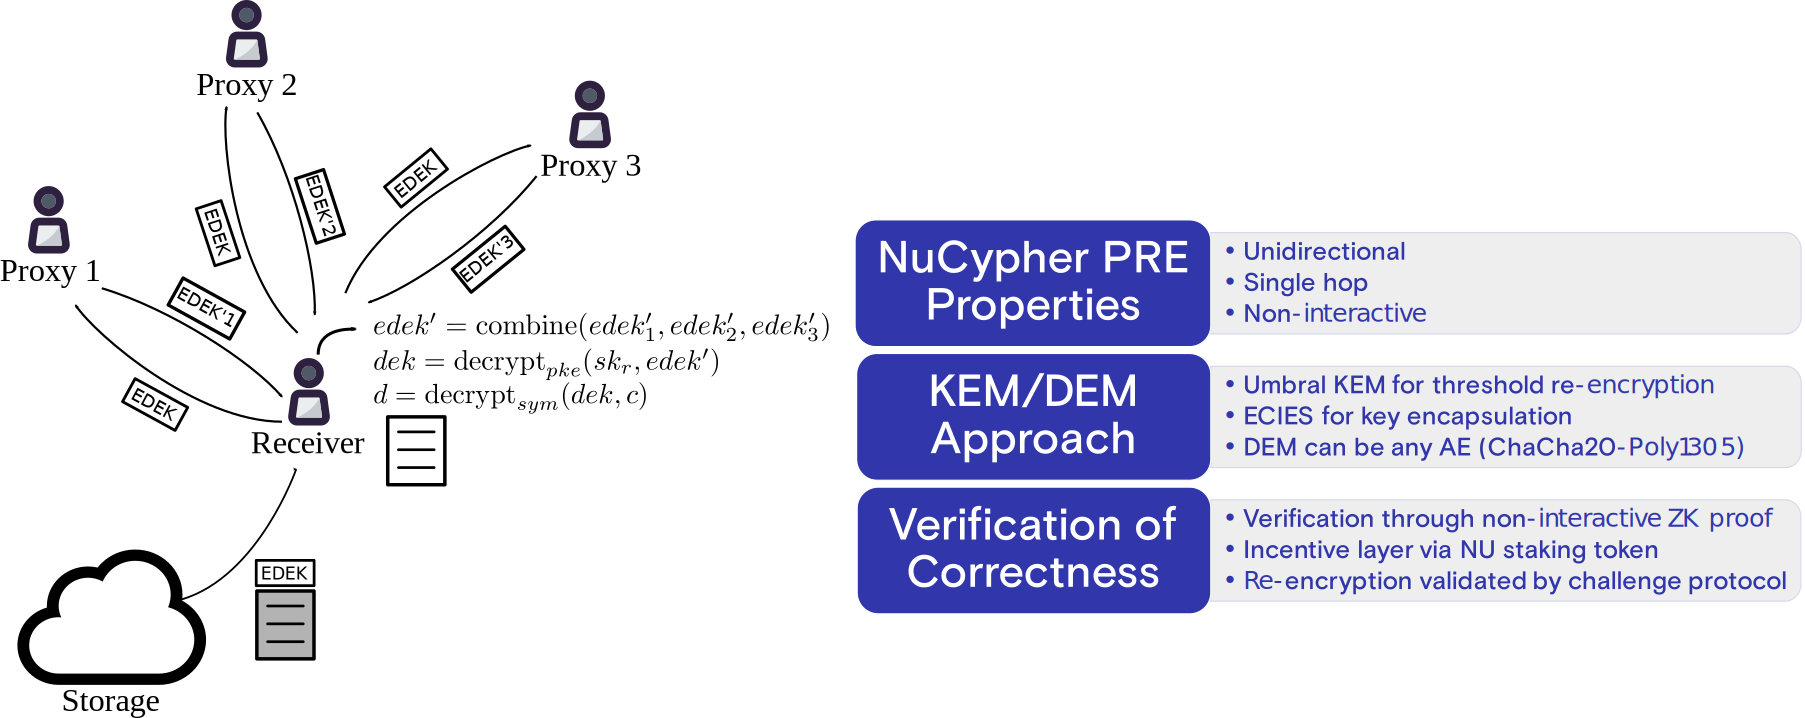
\includegraphics[height=6.5cm]{pdf/decrypt-umbral.pdf}
        \end{figure}
        \url{https://github.com/nucypher/nucypher-kms/}
        \url{https://github.com/nucypher/pyUmbral/}
    \end{frame}

    \begin{frame}
        \frametitle{Sharing in permissioned network}
        \begin{figure}
            \centering
            \includegraphics[height=5.5cm]{pdf/permissioned.pdf}
        \end{figure}
        \begin{itemize}
            \item Node sees everything;
            \item Node can deny to work.
        \end{itemize}
    \end{frame}

    \begin{frame}
        \frametitle{Permissioned network + SSS}
        \begin{figure}
            \centering
            \includegraphics[height=5.5cm]{pdf/permissioned-sss.pdf}
        \end{figure}
        \begin{itemize}
            \item Nodes can collude to see everything.
        \end{itemize}
    \end{frame}

    \begin{frame}
        \frametitle{Sharing with PRE}
        \begin{figure}
            \centering
            \includegraphics[height=5.5cm]{pdf/prenodes.pdf}
        \end{figure}
        \begin{itemize}
            \item Collusion with receiver possible,
            \item Node can deny to work.
        \end{itemize}
    \end{frame}

    \begin{frame}
        \frametitle{Sharing with threshold PRE}
        \begin{figure}
            \centering
            \includegraphics[height=5.5cm]{pdf/umbralnodes.pdf}
        \end{figure}
        \begin{itemize}
            \item Collusion with receiver: $m$ nodes + receiver.
        \end{itemize}
    \end{frame}

    \begin{frame}
        \frametitle{Umbral: threshold proxy re-encryption}
        \begin{itemize}
        	\item \emph{``Umbral''} is Spanish for \emph{``threshold''}
            \item PRE properties: Unidirectional, single-hop, non-interactive
            \item It follows a KEM/DEM approach:
            	\begin{itemize}
					\item UmbralKEM provides the threshold re-encryption capability
                    \item Uses ECIES for key encapsulation with zero knowledge proofs of correctness for verifiability on prime order curves (such as secp256k1)
            		\item The DEM can be any authenticated encryption (currently ChaCha20-Poly1305)
        		\end{itemize}
			\item IND-PRE-CCA security
			\item Verification of re-encryption correctness through Non-Interactive ZK Proofs
			\item Reference implementation: \url{https://github.com/nucypher/pyUmbral/}
			\item Documentation: \url{https://github.com/nucypher/umbral-doc}
        \end{itemize}
    \end{frame}

    \begin{frame}
        \frametitle{Umbral: threshold proxy re-encryption}
        \begin{figure}
            \centering
            \includegraphics[width=11cm]{pdf/umbral-kem-flow.pdf}
        \end{figure}
        \begin{itemize}
			\item Reference implementation: \url{https://github.com/nucypher/pyUmbral/}
			\item Documentation: \url{https://github.com/nucypher/umbral-doc}
        \end{itemize}
    \end{frame}

    \begin{frame}
        \frametitle{Wrapping OpenSSL for EC/BN maths}
        \begin{figure}
            \centering
            \includegraphics[height=7.5cm]{pdf/point.png}
        \end{figure}
    \end{frame}

    \begin{frame}
        \frametitle{Wrapping OpenSSL for EC/BN maths}
        \begin{figure}
            \centering
            \includegraphics[height=7.5cm]{pdf/reencrypt.png}
        \end{figure}
    \end{frame}

    \begin{frame}
        \frametitle{Useful links}
        \begin{figure}
            \centering
            
\includegraphics[width=3cm]{pdf/nucypher_logo.pdf}
        \end{figure}
        Website: \url{https://nucypher.com}

        Github: \url{https://github.com/nucypher/}

        PyUmbral: \url{https://github.com/nucypher/pyUmbral/}

        GoUmbral: \url{https://github.com/nucypher/goUmbral/}

        Mocknet: \url{https://github.com/nucypher/mock-net/}

        Discord: \url{https://discord.gg/7rmXa3S}

        Whitepaper: \url{https://www.nucypher.com/whitepapers/english.pdf}

        E-mail: \url{michael@nucypher.com}

        E-mail: \url{hello@nucypher.com}
    \end{frame}

\end{document}

